
%%%%%%%%%%%%%%%%%%%%%%%%%%%%%%%%%%%%%%%%%%%%
% TODO
% notes on what needs to be done
%%%%%%%%%%%%%%%%%%%%%%%%%%%%%%%%%%%%%%%%%%%%

\documentclass[10pt, letterpaper]{article}
\usepackage[top=0.75in, bottom=0.75in, left=0.75in, right=0.75in]{geometry}

% paragraph spacing
\usepackage[parfill]{parskip}

% Math, graphics, and bibliography
\usepackage{amsmath,amssymb,amsfonts,mathrsfs,mathtools}
\usepackage{graphicx, caption}
\usepackage{floatrow}
\graphicspath{{figures/}}
\usepackage[square,numbers,sort&compress]{natbib}
\usepackage{xcolor}
\renewcommand{\bibnumfmt}[1]{#1.}
\newcommand{\sub}[1]{\ensuremath{_{\textrm{#1}}}}
% \usepackage[square,sort,comma,numbers]{natbib} % my preferred formatting

% for nat biomed eng submission: use line numbers
\usepackage{lineno}
%\linenumbers

% set up using a supplement
\newcommand{\beginsupplement}{%
        \setcounter{table}{0}
        \renewcommand{\thetable}{S\arabic{table}}%
        \setcounter{figure}{0}
        \renewcommand{\thefigure}{S\arabic{figure}}%
     }

\newcommand{\splitcell}[2][c]{%
  \begin{tabular}[#1]{@{}l@{}}#2\end{tabular}}

% My preferred fonts
\usepackage[T1]{fontenc}
\usepackage{lmodern}
\usepackage[sc]{mathpazo}

% For fancier fractions and figure captions
%\usepackage[labelfont={bf}, margin=1cm]{caption}
\usepackage{units}
\setlength{\belowcaptionskip}{15pt plus 3pt minus 2pt}

% \usepackage[utf8]{inputenc}
% \usepackage[english]{babel}
% \usepackage{booktabs}

% \numberwithin{equation}{section}

%\usepackage[document]{ragged2e}
\usepackage{lipsum}

\usepackage{authblk}

\title{TITLE}
\author[1,2,3]{John H. Abel}
\author[1,2,4,5,$\star$]{Emery N. Brown}
\affil[1]{Department of Anesthesiology, Critical Care and Pain Medicine, Massachusetts General Hospital, Boston, MA 02114}
\affil[2]{Picower Institute for Learning and Memory, Massachusetts Institute of Technology, Cambridge, MA 02139}
\affil[3]{Division of Sleep Medicine, Harvard Medical School, Boston, MA 02115}
\affil[4]{Department of Brain and Cognitive Sciences, Massachusetts Institute of Technology, Cambridge, MA 02139}
\affil[5]{Harvard-MIT Health Sciences and Technology, Cambridge, MA 02139}
\affil[$\star$]{Contact: \texttt{enb@neurostat.mit.edu}}
\date{\today}

\begin{document}


\maketitle


\section*{Abstract}
In current anesthesiology practice,

% \section*{Keywords}

\clearpage

\section{Introduction}
Most surgeries are performed under general anesthesia (GA). GA is a reversible, drug-induced state consisting of antinociception, unconsciousness, amnesia, and immobility with maintenance of physiological stability \cite{Brown2010}. 

\section{Results}
See some results in Figure \ref{fig:fig1}.

\section{Discussion}
Despite these successes, there are significant limitations to our approach.




\section{Methods}

\subsection{Datasets}

\subsection{Signal Processing}

\subsection{Classification Models}

\subsection{Statistical Analyses}

\clearpage
\bibliographystyle{myIEEEtran}
\bibliography{condensed_library}


\clearpage

\begin{figure}
\begin{center}
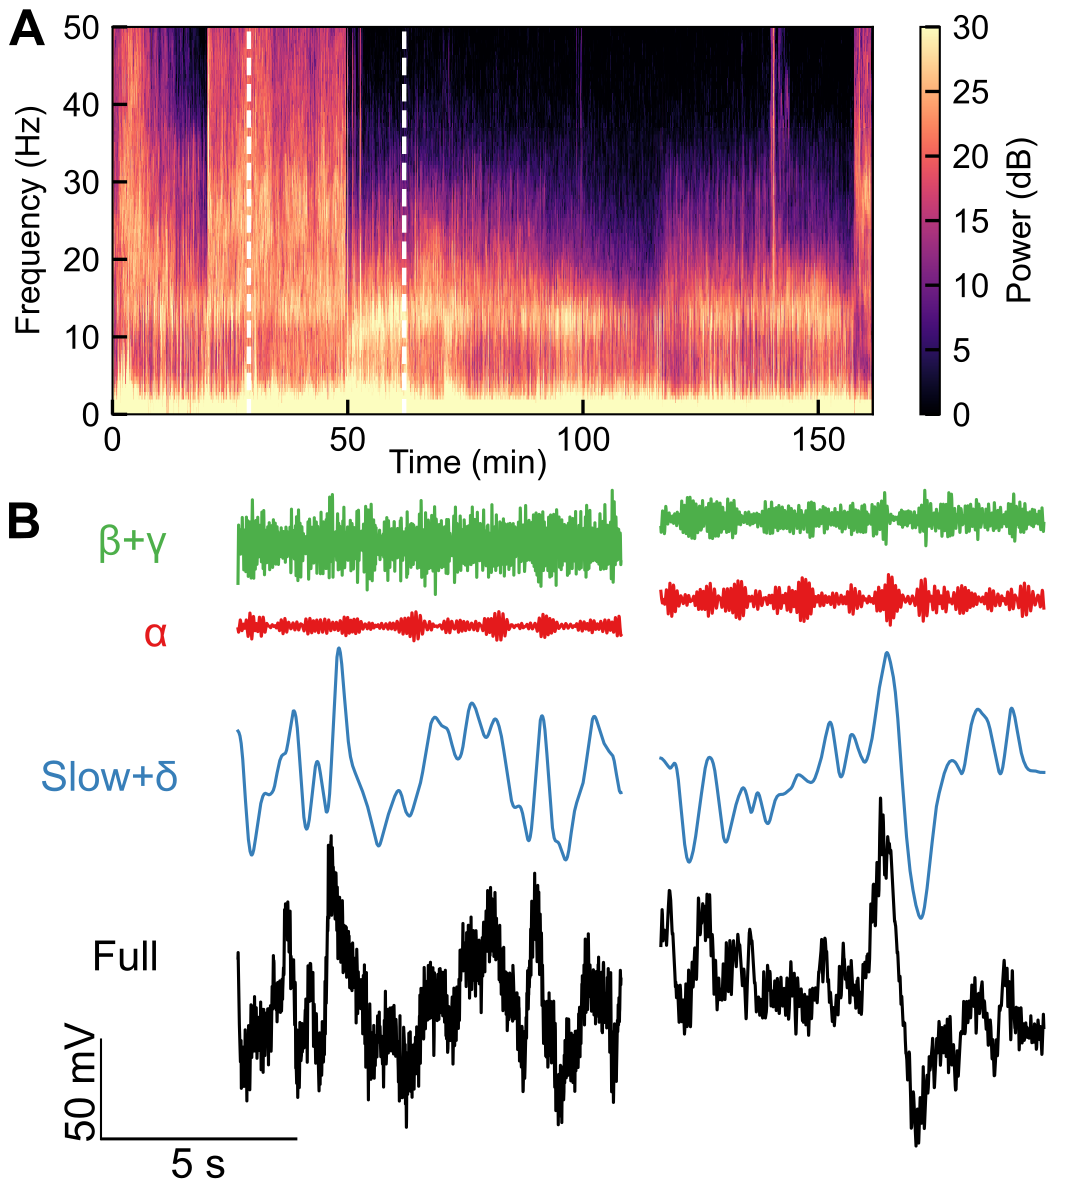
\includegraphics[width=3.5in]{fig1}
\end{center}
\captionsetup{width=3.5in}
\caption{
\label{fig:fig1} An example single-column figure. It looks nice.}
\end{figure}

\beginsupplement

\begin{figure}
  \begin{center}
    %\includegraphics[width=7in]{s1}
    \end{center}
    \captionsetup{width=7in}
    \caption{\label{fig:s1} An example supplemental figure. I didn't put an actual png in here. Still, this is also how to make it two-column.}
\end{figure}

\end{document}

